\documentclass{article}%
\usepackage{amsmath}%
\setcounter{MaxMatrixCols}{30}%
\usepackage{amsfonts}%
\usepackage{amssymb}%
\usepackage{graphicx}
%TCIDATA{OutputFilter=latex2.dll}
%TCIDATA{Version=5.00.0.2552}
%TCIDATA{CSTFile=40 LaTeX article.cst}
%TCIDATA{Created=Wednesday, January 25, 2017 20:51:51}
%TCIDATA{LastRevised=Wednesday, January 25, 2017 22:04:35}
%TCIDATA{<META NAME="GraphicsSave" CONTENT="32">}
%TCIDATA{<META NAME="SaveForMode" CONTENT="1">}
%TCIDATA{<META NAME="DocumentShell" CONTENT="Standard LaTeX\Blank - Standard LaTeX Article">}
%TCIDATA{Language=American English}
\newtheorem{theorem}{Theorem}
\newtheorem{acknowledgement}[theorem]{Acknowledgement}
\newtheorem{algorithm}[theorem]{Algorithm}
\newtheorem{axiom}[theorem]{Axiom}
\newtheorem{case}[theorem]{Case}
\newtheorem{claim}[theorem]{Claim}
\newtheorem{conclusion}[theorem]{Conclusion}
\newtheorem{condition}[theorem]{Condition}
\newtheorem{conjecture}[theorem]{Conjecture}
\newtheorem{corollary}[theorem]{Corollary}
\newtheorem{criterion}[theorem]{Criterion}
\newtheorem{definition}[theorem]{Definition}
\newtheorem{example}[theorem]{Example}
\newtheorem{exercise}[theorem]{Exercise}
\newtheorem{lemma}[theorem]{Lemma}
\newtheorem{notation}[theorem]{Notation}
\newtheorem{problem}[theorem]{Problem}
\newtheorem{proposition}[theorem]{Proposition}
\newtheorem{remark}[theorem]{Remark}
\newtheorem{solution}[theorem]{Solution}
\newtheorem{summary}[theorem]{Summary}
\newenvironment{proof}[1][Proof]{\noindent\textbf{#1.} }{\ \rule{0.5em}{0.5em}}
\begin{document}

\title{IPB Reactor Calorimetry Coefficient of Performance (COP) Note}
\author{Jin Liu }
\date{January 25, 2017}
\maketitle

Definitions

$P$ power deposit to the core either by $DC$ or $Q$-pulse in watts

$Hpdrop$ \ heater power drop after power deposit to the core in watts

$V_{1}$ voltage measured at the core entrance

$V_{2}$ voltage measured at the core exit

$V^{2}=(V_{1}-V_{2})^{2}$%


\begin{equation}
C=\frac{Hpdrop}{V^{2}}[watts/volts^{2}], [watts/volts^{2}] = 1/[ohms] \label{1}%
\end{equation}
%
Where C is constant at any given core temperature of power DC or $Q$-pulse, gas hydrogen or helium of ipb1-30b and sri-ipb2-27b. 
 
\begin{equation}
R=\frac{V^{2}}{P}\ [volts^{2}/watts], [volts^{2}/watts]=[ohms]\label{2}%
\end{equation}
%
Where R is constant at any given core temperature for all DC.
\begin{equation}
cop=\frac{Hpdrop_{^{Q}}(P)-Hpdrop_{^{DC}}(P)}{P}\label{3}%
\end{equation}


For any given $V_{DC}^{2}$,
\begin{align}
cop & =\frac{Hpdrop_{^{Q}}-Hpdrop_{^{DC}}}{P}=\frac{C_{Q}V_{DC}^{2}%
-C_{DC}V_{DC}^{2}}{P_{DC}}\nonumber\\
& =\frac{C_{Q}V_{DC}^{2}-C_{DC}V_{DC}^{2}}{V_{DC}^{2}/R_{DC}}=\left(
C_{Q}-C_{DC}\right)  R_{DC}\label{5}%
\end{align}

\begin{figure}
[h]
\begin{center}
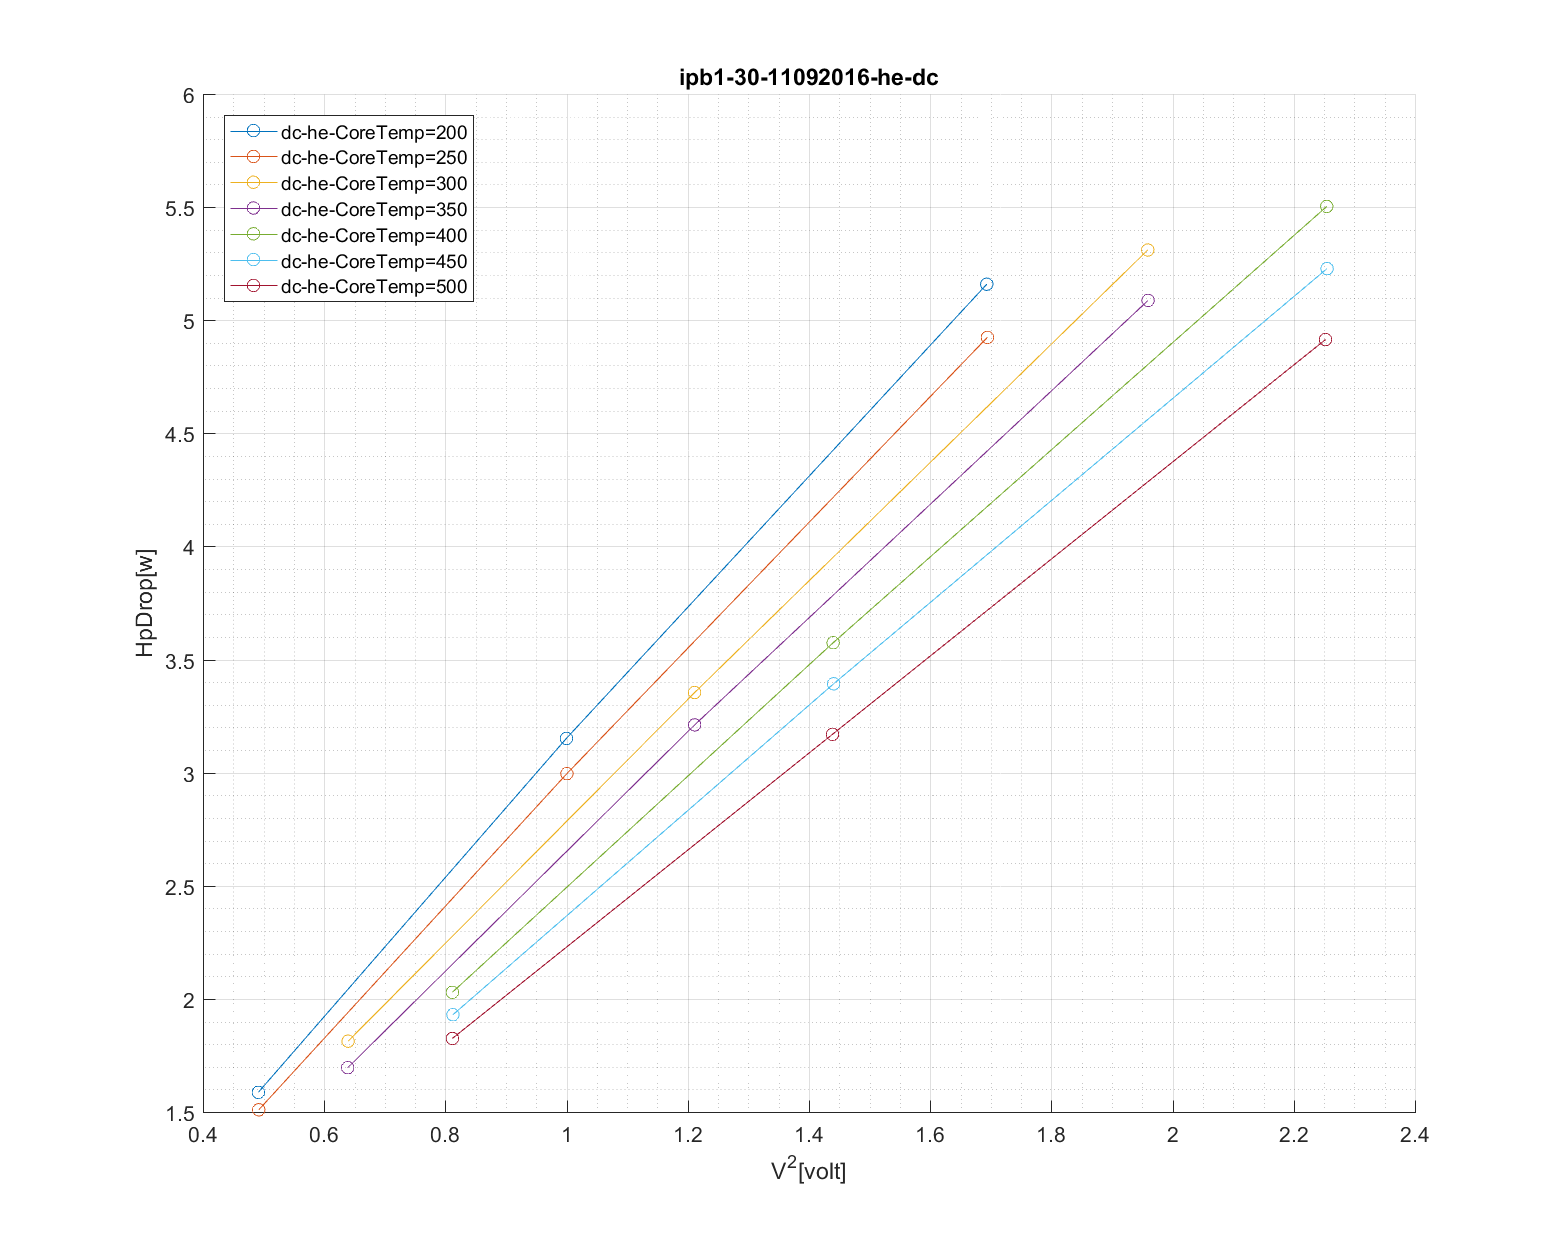
\includegraphics[scale=0.4]{ipb1-30-11092016-he-dc-HpD-V2.png} 
\caption{Inner Core Temperature and Heat Power vs. Running Hours}%
\end{center}
\end{figure}
\begin{figure}
[h]
\begin{center}
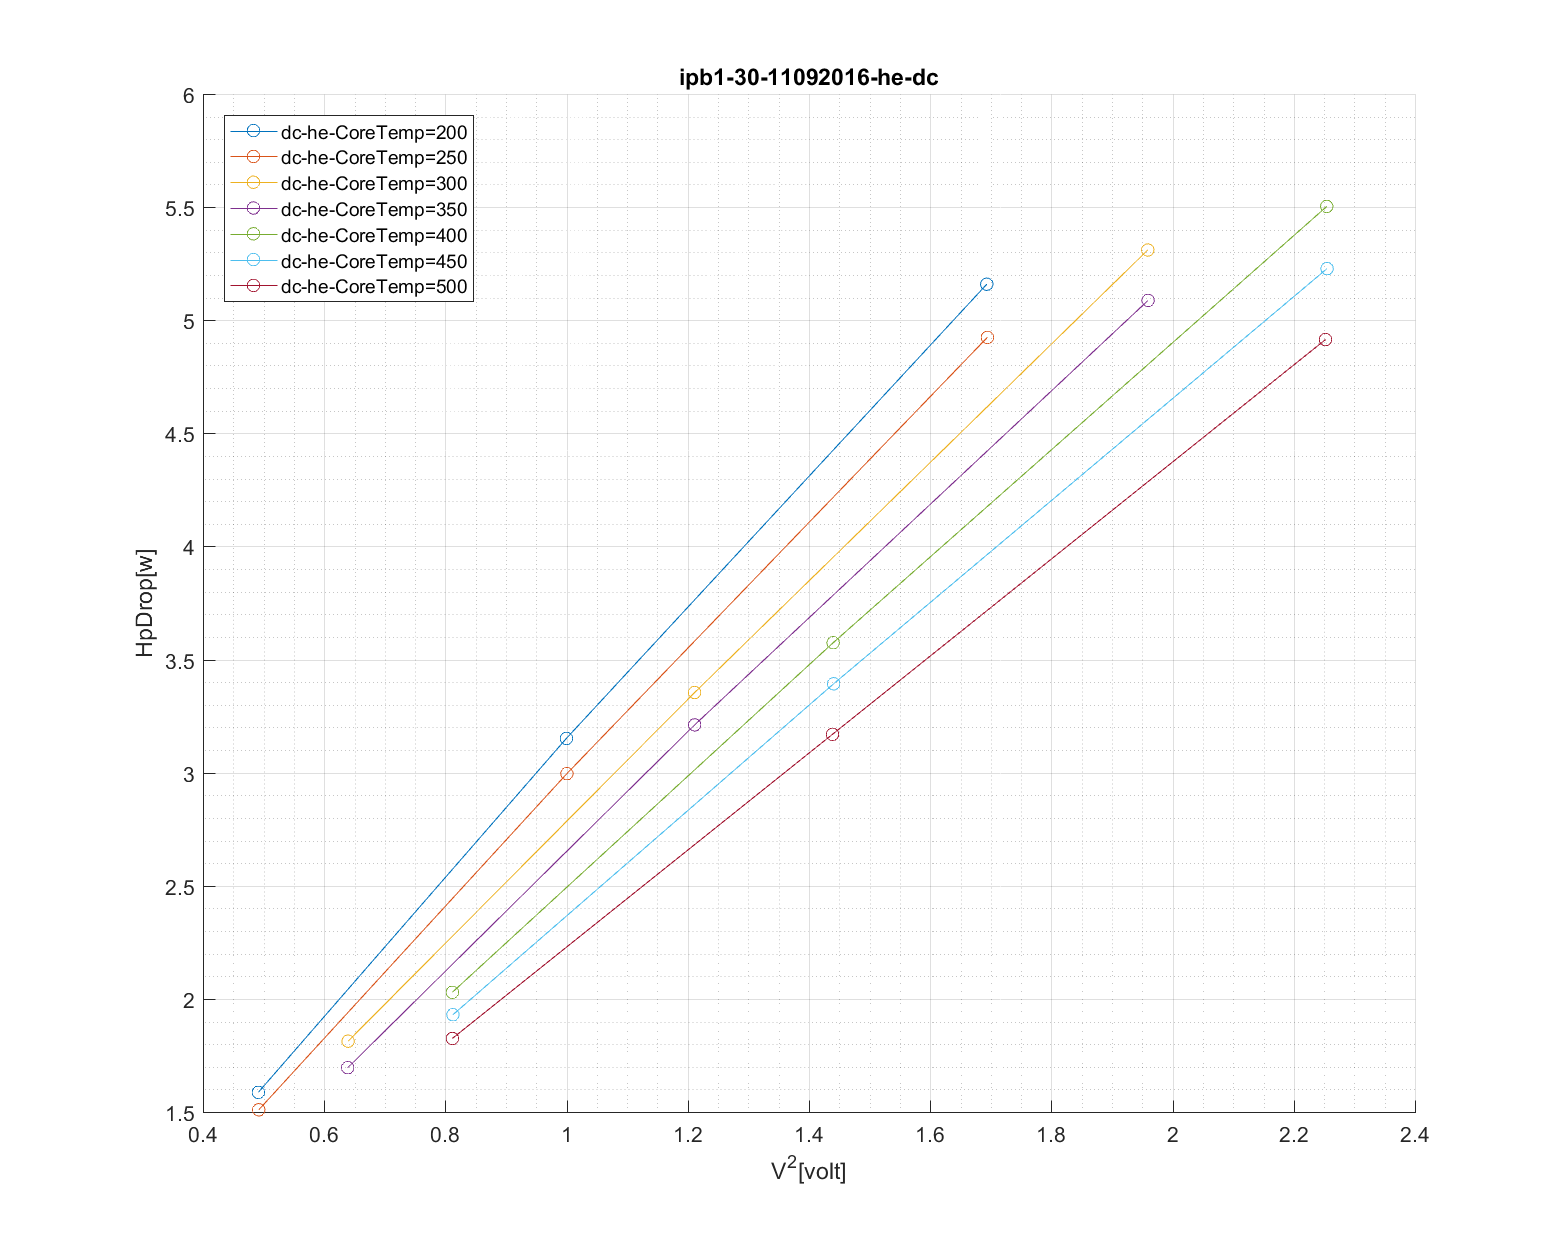
\includegraphics[scale=0.4]{ipb1-30-11092016-he-dc-HpD-V2.png} 
\caption{Inner Core Temperature and Heat Power vs. Running Hours}%
\end{center}
\end{figure}



\end{document}